% ===========================================================================
% SE-490 Cloud Computing - Complex Engineering Activity (CEA)
% Technical report: OccasionHub three-tier deployment on AWS
%
% Compile: pdflatex main.tex  (run twice for references)
%   or upload the "report" folder to Overleaf and press Recompile.
% Screenshots: drop PNG files into figures/ with the names listed in
%   Appendix A; missing ones show as labelled placeholder boxes.
% All placeholders filled on 8 Nov 2026 from the live deployment.
% ===========================================================================
\documentclass[10pt,a4paper]{article}

\usepackage[utf8]{inputenc}
\usepackage[T1]{fontenc}
\usepackage{lmodern}
\usepackage[a4paper,margin=1.8cm]{geometry}
\usepackage{microtype}
\usepackage{graphicx}
\usepackage{booktabs}
\usepackage{tabularx}
\usepackage{array}
\usepackage{float}
\usepackage[font=small,labelfont=bf]{caption}
\usepackage[dvipsnames,table]{xcolor}
\usepackage{enumitem}
\usepackage{amssymb}
\usepackage[hidelinks]{hyperref}

\setlist{nosep,leftmargin=1.4em}
\setlength{\parskip}{0.35em}
\setlength{\parindent}{0pt}
\renewcommand{\arraystretch}{1.18}
\newcolumntype{L}{>{\raggedright\arraybackslash}X}

% ---- Details to fill in ---------------------------------------------------
\newcommand{\fillin}[1]{\textcolor{red}{\textbf{[#1]}}}
\newcommand{\student}{Ali Afzal (SE-23048)}
\newcommand{\repourl}{\url{https://github.com/Woodenbowl000/occasionhub-cloud}}
\newcommand{\appurl}{\url{http://occasionhub-public-alb-777768551.ap-southeast-2.elb.amazonaws.com}}

% Screenshot evidence: the image if present, otherwise a placeholder box
\newcommand{\evidence}[3]{%
  \begin{figure}[H]\centering
  \IfFileExists{figures/#1}%
    {\includegraphics[width=\linewidth,height=0.36\textheight,keepaspectratio]{figures/#1}}%
    {\fbox{\parbox[c][3.2cm][c]{0.92\linewidth}{\centering\small
      \textcolor{red}{Screenshot to add: \texttt{figures/#1}}\\[2pt] #2}}}%
  \caption{#2}\label{#3}
  \end{figure}}

\begin{document}

% ---- Title block -----------------------------------------------------------
\begin{center}
{\LARGE\bfseries Design, Deployment and Cloud-Native Enhancement\\[2pt]
of a Three-Tier Web Application on AWS}\\[6pt]
{\large OccasionHub: event-venue booking platform}\\[8pt]
SE-490 Cloud Computing \textperiodcentered{} Complex Engineering Activity
\textperiodcentered{} Department of Software Engineering\\[3pt]
\student\\[3pt]
Source code: \repourl\\[2pt]
\today
\end{center}
\vspace{-0.4em}
\noindent\rule{\linewidth}{0.4pt}

% ===========================================================================
\section{Introduction and choice of cloud provider}
% ===========================================================================
OccasionHub is our venue-booking web application (search venues by city, type,
price and distance; negotiate and book; admin approval), previously hosted on
Vercel and Neon. We containerised it and deployed it on \textbf{AWS}
(\texttt{ap-southeast-2}, Sydney) as three tiers: an Nginx + Next.js 15 \emph{web tier}, an
Express + Prisma \emph{application tier} (Node.js 22), and an Amazon RDS
PostgreSQL 16 \emph{database tier}. Terraform defines the environment and GitHub
Actions releases it.

\textbf{Why AWS.} Every requirement maps to a mature native service (VPC, ALB,
EC2 Auto Scaling, RDS, ECR, Secrets Manager, CloudWatch). RDS PostgreSQL supports
\emph{PostGIS}, which the app needs for venue coordinates and distance search.
GitHub Actions has first-party AWS actions for credentials and ECR.
The Terraform AWS provider covers every resource, so the stack is created and
destroyed with one command. Free Tier credits cover the t3.micro and
db.t4g.micro instances.

% ===========================================================================
\section{Overall architecture and design decisions}
% ===========================================================================
Figure~\ref{fig:arch} shows the deployed system. A user's request enters
through the Internet Gateway to the internet-facing ALB, which forwards it to a
web-tier instance. Nginx serves the Next.js pages and forwards every
\texttt{/backend/*} call to an \emph{internal} ALB. The internal ALB balances
requests over the application instances, which query RDS over TLS. Nothing
behind the public ALB has a public IP address.

\begin{figure}[!t]
  \centering
  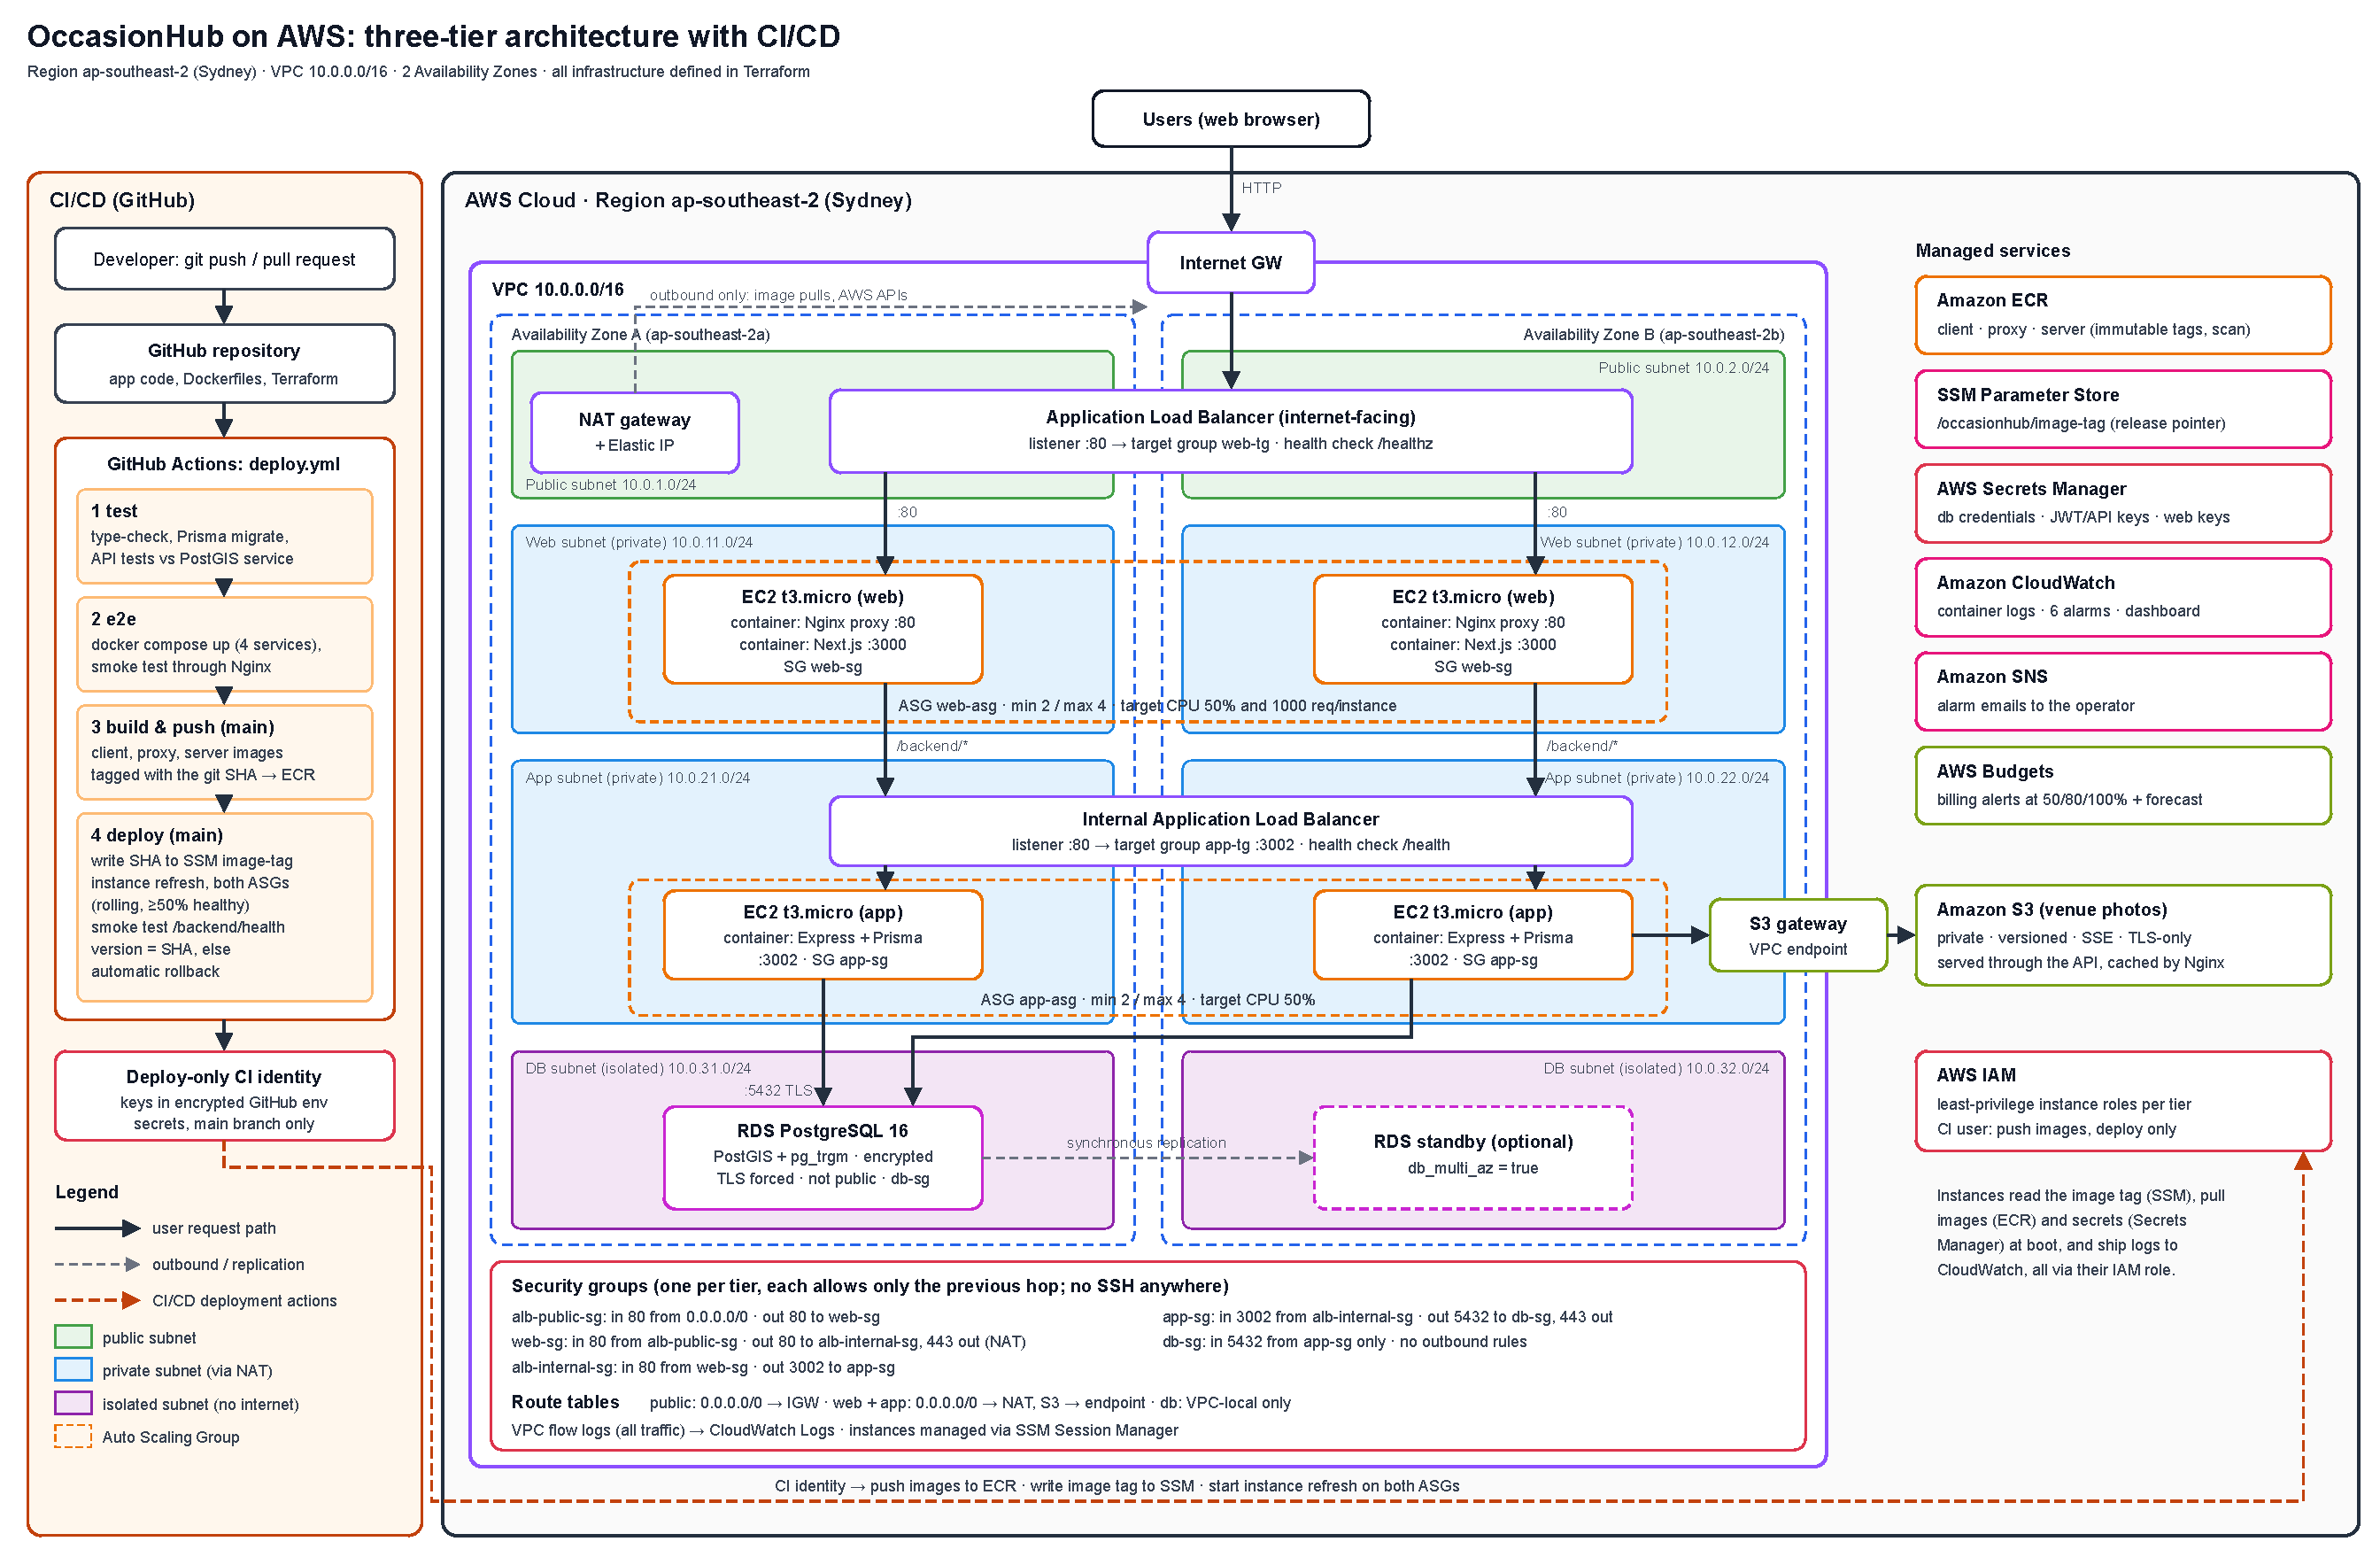
\includegraphics[width=\linewidth]{figures/architecture.pdf}
  \caption{Deployed architecture: network layers, both Availability Zones,
  load balancers, Auto Scaling Groups, managed services, security groups and the
  CI/CD flow (source: \texttt{docs/architecture.svg}).}
  \label{fig:arch}
\end{figure}

\textbf{Network design.} One VPC (\texttt{10.0.0.0/16}) spans two Availability
Zones (AZs). Each AZ has four /24 subnets, one per layer, so every tier is
isolated by routing as well as by firewall rules (Table~\ref{tab:net}).

\begin{table}[H]\centering\small
\caption{Subnets and routing (identical layout in AZ A and AZ B).}\label{tab:net}
\begin{tabularx}{\linewidth}{@{}l l L L@{}}
\toprule
Layer & CIDR (AZ A / AZ B) & Default route & Contents \\
\midrule
Public & 10.0.1.0/24, 10.0.2.0/24 & Internet Gateway & internet-facing ALB, NAT gateway \\
Web (private) & 10.0.11.0/24, 10.0.12.0/24 & NAT gateway; S3 via gateway endpoint & web-tier EC2 instances (ASG) \\
App (private) & 10.0.21.0/24, 10.0.22.0/24 & NAT gateway; S3 via gateway endpoint & internal ALB, app-tier EC2 instances (ASG) \\
DB (isolated) & 10.0.31.0/24, 10.0.32.0/24 & none (VPC-local only) & RDS PostgreSQL (and optional standby) \\
\bottomrule
\end{tabularx}
\end{table}

\textbf{Key design decisions.}
\begin{itemize}
  \item \textbf{Two load balancers:} the API sits behind an \emph{internal} ALB,
  so it is never reachable from the internet, and it gets its own target group,
  health checks and scaling.
  \item \textbf{Same-origin API:} the browser calls \texttt{/backend/...} and
  Nginx proxies it. There is no CORS on the request path and no API hostname
  baked into the bundle, so the same image runs locally and in the cloud.
  \item \textbf{Stateless instances:} photos go to S3 and sessions are JWTs,
  so any instance can be added, replaced or removed at any time.
  \item \textbf{Immutable releases:} images are tagged with the git SHA, and the
  SSM parameter \texttt{/occasionhub/image-tag} names the live release. A deploy
  means ``change the pointer, replace instances''.
  \item \textbf{EC2 + Docker, not Kubernetes:} the simplest platform that meets
  every requirement on Free Tier-sized instances; the containers can move to ECS
  or EKS unchanged.
\end{itemize}

% ===========================================================================
\section{Services used and their role in each tier}
% ===========================================================================
\begin{table}[H]\centering\small
\caption{AWS services and their role.}\label{tab:services}
\begin{tabularx}{\linewidth}{@{}l L@{}}
\toprule
Service & Role in the solution \\
\midrule
VPC, subnets, IGW, NAT gateway, route tables & Network layer described in Table~\ref{tab:net}; NAT gives private instances outbound-only access (image pulls, AWS APIs). \\
Application Load Balancer $\times$2 & Public ALB $\rightarrow$ web target group (port 80, health check \texttt{/healthz}); internal ALB $\rightarrow$ app target group (port 3002, \texttt{/health}). \\
EC2 + Auto Scaling Groups & Amazon Linux 2023 t3.micro instances from launch templates; web and app ASGs (min 2, max 4) across both AZs with target-tracking policies. \\
Amazon RDS for PostgreSQL 16 & Managed database in the isolated subnets: encrypted gp3 storage, automated backups, forced TLS, slow-query log; optional Multi-AZ standby. \\
Amazon ECR & Private registry, one repository per image (\texttt{client}, \texttt{proxy}, \texttt{server}); immutable tags, scan on push, keep the last 10 images. \\
AWS Secrets Manager & Database credentials, JWT signing key and optional Stripe, Google and Resend keys; read at container start through the instance role. \\
SSM Parameter Store & Release pointer \texttt{/occasionhub/image-tag} written by the pipeline. \\
Amazon S3 + gateway endpoint & Private, versioned, encrypted bucket for venue photos; reached without the NAT through a free gateway endpoint. \\
CloudWatch, SNS & Container and VPC flow logs, 6 alarms, one dashboard; alarm and recovery emails through SNS. \\
AWS Budgets & Billing alerts at 50\%, 80\% and 100\% of a monthly limit, plus a forecast alert. \\
IAM & Least-privilege role per tier; a deploy-only CI identity for GitHub Actions. Instances are managed with SSM Session Manager; no SSH. \\
\bottomrule
\end{tabularx}
\end{table}

% ===========================================================================
\section{Containerisation and CI/CD pipeline}
% ===========================================================================
\textbf{Images.} Each tier has a multi-stage Dockerfile. The final images are
slim, run as non-root users and define a \texttt{HEALTHCHECK}.
\begin{itemize}
  \item \texttt{server/}: compiles TypeScript and the Prisma client, then ships
  only production dependencies, with \texttt{tini} for graceful shutdown. Its
  entrypoint loads secrets, runs \texttt{prisma migrate deploy} (safe from many
  instances because it takes a lock), optionally seeds data, then starts the API.
  \item \texttt{client/}: Next.js \emph{standalone} output; the runtime holds
  56\,MB instead of 643\,MB of \texttt{node\_modules}.
  \item \texttt{proxy/}: \texttt{nginx-unprivileged}, with its configuration
  rendered from environment variables at start.
\end{itemize}
\texttt{docker-compose.yml} runs db, server, client and proxy on three networks
(\texttt{web}, \texttt{app}, \texttt{data}) that mirror the cloud segmentation.

\textbf{Pipeline} (\texttt{.github/workflows/deploy.yml}):
\begin{enumerate}
  \item \textbf{test} (every push and pull request): type-check, migrate and
  seed a PostGIS service container, then run 11 API tests.
  \item \textbf{e2e}: \texttt{docker compose up --build --wait}, then smoke-test
  the pages, the API and venue search through Nginx.
  \item \textbf{build-push} (\texttt{main} only): a matrix job pushes the three
  images to ECR, tagged with the SHA and built with the layer cache.
  \item \textbf{deploy} (\texttt{main}, environment \texttt{production}):
  \texttt{scripts/deploy.sh} writes the SHA to the release pointer and starts an
  \emph{instance refresh} on both ASGs, so new instances must pass ALB health
  checks while at least 50\% keep serving. It then checks that
  \texttt{/backend/health} reports the new SHA. On failure it restores the
  previous tag and refreshes again (automatic rollback).
\end{enumerate}

% ===========================================================================
\section{Security considerations}\label{sec:sec}
% ===========================================================================
\begin{itemize}
  \item \textbf{Security groups:} one per tier, each admitting only the previous
  hop by security-group reference: internet $\rightarrow$ public ALB :80
  $\rightarrow$ web :80 $\rightarrow$ internal ALB :80 $\rightarrow$ app :3002
  $\rightarrow$ database :5432. Egress is explicit; the database has none. No
  SSH anywhere; operators use SSM Session Manager.
  \item \textbf{Segmentation:} only the ALB and NAT are public. Web and app
  instances have no public IPs. Database subnets have no internet route, and RDS
  is not publicly accessible. VPC flow logs record all traffic.
  \item \textbf{Secrets:} Terraform generates the database password and JWT key
  into Secrets Manager. Containers read them at start through the instance role,
  so nothing secret is in images, launch templates, user data or git. Locally,
  values come from a git-ignored \texttt{.env}.
  \item \textbf{Pipeline:} keyless OIDC federation was the first choice, but
  the AWS-managed service control policy of our new-experience (Free plan)
  project denies \texttt{iam:*Provider*}, so no identity provider can be
  created. The pipeline therefore uses a dedicated IAM user with no console
  password and one inline policy: push to three ECR repositories, write one
  parameter, refresh \texttt{occasionhub-*} ASGs. Its keys are encrypted GitHub
  \emph{environment} secrets of \texttt{production}, which only the
  \texttt{main} branch can use, and are masked in logs. The secret exists only in
  the Terraform state, which is kept outside the project folder, and is rotated
  with one \texttt{terraform apply -replace}. Setting \texttt{github\_auth\_mode = "oidc"}
  restores keyless login on an account that allows it.
  \item \textbf{Least-privilege roles:} the web role reads only its images, the
  release pointer and the web secret. The app role adds the database and app
  secrets and \texttt{venues/*} in the photo bucket.
  \item \textbf{Encryption and hardening:} at rest on RDS, EBS, S3 and ECR. TLS
  is forced to RDS (\texttt{rds.force\_ssl=1}) and S3 (deny non-TLS policy).
  Instances require IMDSv2, containers run as non-root, ALBs drop invalid
  headers, Nginx adds security headers, and images are scanned on push.
  \item \textbf{Application fixes:} venue sorting now accepts only a fixed set
  of columns, page size is capped at 100, and photo names are validated before
  being read from S3.
\end{itemize}

% ===========================================================================
\section{Cloud-native enhancements}
% ===========================================================================
Five enhancements were implemented:
\begin{itemize}
  \item \textbf{Infrastructure as code:} about 1{,}700 lines of Terraform, validated.
  \item \textbf{Object storage:} S3 for venue photos.
  \item \textbf{Persistent block storage:} encrypted gp3 EBS volumes for
  instances and RDS (storage auto-scaling is one variable away; off by default
  to stay within the Free Tier's 20\,GB).
  \item \textbf{Centralised logging and monitoring:} CloudWatch.
  \item \textbf{Cost estimate and optimisation:} Tables~\ref{tab:cost}
  and~\ref{tab:costopt}.
\end{itemize}

\textbf{Monitoring.} Docker's \texttt{awslogs} driver streams every container to
CloudWatch Logs, and RDS exports statements slower than 500\,ms. Six alarms email
through SNS: ALB 5xx errors, p95 latency above 1\,s, unhealthy hosts per tier,
database CPU and database storage. A dashboard shows traffic, latency, CPU per
tier, instances in service, healthy targets and recent API errors.

\textbf{Cost estimate.} Table~\ref{tab:cost} uses AWS on-demand prices for
\texttt{ap-southeast-2} (Sydney), 730 hours a month and light traffic. Unit prices were retrieved from the
AWS Price List API (\texttt{aws pricing get-products}) on \today.

\begin{table}[H]\centering\small
\caption{Estimated monthly cost (USD), default configuration.}\label{tab:cost}
\begin{tabularx}{\linewidth}{@{}L r@{}}
\toprule
Item & USD / month \\
\midrule
4 $\times$ EC2 t3.micro (2 web + 2 app), \$0.0132/h & 38.54 \\
4 $\times$ 20\,GB gp3 EBS (\$0.096/GB) & 7.68 \\
2 $\times$ Application Load Balancer (\$0.0252/h + about 0.5 LCU each) & 42.63 \\
NAT gateway (\$0.059/h + 10\,GB processed) & 43.66 \\
3 public IPv4 addresses (2 on the ALB, 1 on the NAT) & 10.95 \\
RDS db.t4g.micro single-AZ (\$0.025/h) + 20\,GB gp3 (\$0.138/GB) & 21.01 \\
Secrets Manager (3 secrets), CloudWatch logs, S3, ECR & 4.20 \\
\midrule
\textbf{Total, about \$0.23 per hour} & \textbf{168.67} \\
\bottomrule
\end{tabularx}
\end{table}

\begin{table}[H]\centering\small
\caption{Cost optimisation measures.}\label{tab:costopt}
\begin{tabularx}{\linewidth}{@{}L r L@{}}
\toprule
Measure & Saving / month & Trade-off \\
\midrule
Run only while needed: deploy, collect evidence, \texttt{terraform destroy} (implemented: whole stack is code; billing alerts via AWS Budgets) & up to 100\% & recreation takes about 15 min \\
1-year Compute Savings Plan + RDS reserved instance & about \$20 (30--40\% of EC2/RDS) & 1-year commitment \\
Graviton (t4g.micro) with multi-arch images (buildx) & about \$8 (20\% of EC2) & arm64 build stage in CI \\
Scheduled scaling to 1 instance per tier at night (ASG scheduled actions) & about \$10 & no redundancy during those hours \\
NAT instance (t4g.nano) instead of NAT gateway, dev only & about \$39 & self-managed, lower throughput \\
\bottomrule
\end{tabularx}
\end{table}

\textbf{Application performance.} Moving to the cloud exposed four
inefficiencies, now fixed:
\begin{itemize}
  \item \textbf{N+1 query:} venue search ran one PostGIS query per venue (24
  sequential database round trips for 20 venues); it now uses one batched query
  plus a parallel count (5 round trips).
  \item \textbf{Missing indexes:} a migration adds a trigram index for city
  search, a GIST spatial index and three B-tree indexes.
  \item \textbf{Payload size:} the API gzips JSON, and lazy-loading the Mapbox
  map cut \texttt{/venues} first-load JavaScript from 676\,kB to 237\,kB.
  \item \textbf{Edge caching:} Nginx compresses text and caches content-hashed
  assets and photos.
\end{itemize}

% ===========================================================================
\section{Testing results}\label{sec:test}
% ===========================================================================
\textbf{Local verification (\today).} All 11 API tests pass against
PostgreSQL + PostGIS: liveness and readiness, venues with coordinates, gzip,
page-size cap and sort whitelist, distance order, case-insensitive city search,
admin sign-in returns a JWT, and wrong password rejected. Also confirmed:
\begin{itemize}
  \item migrations apply cleanly and the seed script is idempotent;
  \item \texttt{EXPLAIN} shows city search using the trigram index;
  \item \texttt{terraform validate} succeeds and the rendered user-data scripts
  pass \texttt{bash -n};
  \item Nginx passed \texttt{nginx -t} and a live run in front of the built
  front end and API: \texttt{/backend} routing, gzip, single security headers,
  and static-asset cache \texttt{MISS}$\rightarrow$\texttt{HIT}.
\end{itemize}

\begin{table}[H]\centering\small
\caption{Venue search, before and after optimisation (1{,}000 requests, concurrency 10, 20 venues per page).}\label{tab:bench}
\begin{tabularx}{\linewidth}{@{}L r r r@{}}
\toprule
Variant & Requests/s & p50 latency (ms) & p95 latency (ms) \\
\midrule
Before (N+1 coordinate queries) & 108--218 & 46--88 & 60--129 \\
After (batched query, parallel count) & 391--410 & 23--24 & 33--36 \\
\bottomrule
\end{tabularx}
\end{table}

\textbf{Automated deployment on AWS (8 Nov 2026).} Pushing commit
\texttt{e7f505a}, a visible change to the landing-page tagline, to
\texttt{main} triggered pipeline run \#4 (Table~\ref{tab:run}). The first deploy
attempt stopped at its pre-flight check after 12\,s because the
\texttt{APP\_URL} repository variable was not yet set. No AWS resource was
changed, so the safety check worked as designed. After the variable was added,
re-running the failed job replaced all four instances with the new release while
the site stayed up. \texttt{/backend/health} then reported \texttt{e7f505a} at
\appurl{} (taken down after evaluation to save cost). Of 24 consecutive requests,
the two web instances answered 12 and 12 (\texttt{X-Served-By}) and the two app
instances 13 and 11 (\texttt{X-App-Instance}), which confirms load balancing in
both tiers (Figures~\ref{fig:gha}--\ref{fig:app}).

\begin{table}[H]\centering\small
\caption{Pipeline run \#4 for commit \texttt{e7f505a} (GitHub Actions).}\label{tab:run}
\begin{tabularx}{\linewidth}{@{}L l r@{}}
\toprule
Job & Result & Duration (m:ss) \\
\midrule
Test API against PostgreSQL + PostGIS & passed & 0:43 \\
Build all images + end-to-end smoke test (docker compose) & passed & 2:06 \\
Build \& push server / client / proxy (in parallel) & passed & 0:28 / 1:33 / 0:31 \\
Deploy: release pointer, rolling refresh of both ASGs, smoke test & passed & 6:54 \\
\bottomrule
\end{tabularx}
\end{table}

% ===========================================================================
\section{Non-functional requirements}\label{sec:nfr}
% ===========================================================================
\begin{table}[H]\centering\small
\caption{How the design meets each NFR, and what it does not yet address.}\label{tab:nfr}
\begin{tabularx}{\linewidth}{@{}>{\raggedright\arraybackslash\bfseries}p{2.55cm} L L@{}}
\toprule
NFR & Design decisions that support it & Known limitations / improvement \\
\midrule
Scalability & Stateless containers (JWT sessions, photos in S3); separate ASGs and target groups per tier scale independently up to 4 instances each; batched queries and indexes reduce per-request database load. & Single RDS instance limits write scale; add read replicas, RDS Proxy for connection pooling, and Redis for caching. \\
Availability / Reliability & Two AZs for every layer; at least 2 instances per tier; ALB health checks and ELB-type ASG health checks replace failed instances automatically; rolling deploys keep at least 50\% serving; automatic rollback; daily RDS backups. & RDS single-AZ and a single NAT gateway by default (cost). Set \texttt{db\_multi\_az = true} and \texttt{single\_nat\_gateway = false} for production. \\
Elasticity & Target tracking on CPU (50\%) for both tiers and on ALB requests per target for the web tier, so capacity grows and shrinks automatically between min and max; RDS storage auto-scaling can be enabled (\texttt{db\_max\_allocated\_storage}). & New instances take about 2--3 minutes (package install and image pull); a pre-baked AMI or ECS on Fargate would react faster. \\
Security & See Section~\ref{sec:sec}: per-tier security groups, isolated database subnets, Secrets Manager, branch-restricted deploy-only CI identity, least-privilege IAM, encryption, IMDSv2, non-root containers, flow logs. & HTTP only: no domain or certificate (add ACM + HTTPS listener and AWS WAF). CI uses long-lived keys because the project SCP blocks OIDC: rotate them, or switch to OIDC on an advanced account. \\
Maintainability / Deployability & One command builds the infrastructure; every push is tested, built, deployed and verified without manual steps; immutable SHA-tagged images make each release traceable and reversible; identical containers locally and in the cloud. & Terraform runs manually with local state; move state to S3 with locking and add a plan/apply pipeline. \\
Performance / Latency & Nginx gzip and caching; static assets cached for a year; smaller JavaScript bundle; N+1 query removed (median latency 46--88\,ms to about 24\,ms); keep-alive tuned above the ALB idle timeout; same-region placement of all tiers. & No CDN; Amazon CloudFront in front of the ALB would cut latency for distant users. \\
Cost-Efficiency & Free Tier-sized instances; scaling to the minimum when idle; S3 gateway endpoint avoids NAT data charges; 14-day log retention; ECR lifecycle policy; billing alerts; whole stack destroyable (Table~\ref{tab:costopt}). & Fixed hourly costs (2 ALBs, NAT) dominate at low traffic; a single-host deployment would cost far less for a demo. \\
Portability & Every tier is a standard OCI container; configuration only through environment variables; the same images run with docker compose, on EC2, or on ECS, EKS or another cloud's VMs; PostgreSQL is open source. & AWS-specific glue (Secrets Manager loader, S3 client, Terraform) would need a provider swap; Kubernetes manifests would ease that move. \\
\bottomrule
\end{tabularx}
\end{table}

% ===========================================================================
\section{Conclusion}
% ===========================================================================
OccasionHub now runs on AWS as a segmented, horizontally scalable three-tier
system. Infrastructure, images and releases are all reproducible from the git
repository. A push to \texttt{main} tests the code, builds and publishes three
images, rolls them out across two Availability Zones without downtime, and
verifies the result. The migration also made the application measurably faster.

The main gaps are HTTPS, a Multi-AZ database and remote Terraform state. Each
is a configuration change, not a redesign.

% ===========================================================================
\clearpage
\appendix
\section*{Appendix A: Deployment evidence}
\addcontentsline{toc}{section}{Appendix A: Deployment evidence}
% ===========================================================================
All figures were captured on 8 Nov 2026 from the live deployment in the AWS
Management Console (\texttt{ap-southeast-2}), the public GitHub Actions run and
the live site.

\evidence{aws-vpc-subnets.png}{VPC \texttt{occasionhub-vpc} with its eight subnets across two AZs.}{fig:vpc}
\evidence{aws-route-tables.png}{Route tables: one public, one private per AZ and one isolated database table, each associated with two subnets.}{fig:rt}
\evidence{aws-ec2-instances.png}{EC2 instances: two web and two app instances running in two AZs, all status checks passed, no public IPv4 address.}{fig:ec2}
\evidence{aws-asg.png}{Auto Scaling Groups \texttt{occasionhub-web-asg} and \texttt{occasionhub-app-asg} with target-tracking policies.}{fig:asg}
\evidence{aws-security-groups.png}{Security group \texttt{occasionhub-db-sg}: one inbound rule (PostgreSQL 5432, from the application tier only) and no outbound rules.}{fig:sg}
\evidence{aws-load-balancers.png}{Target group \texttt{occasionhub-web-tg} behind the public ALB: both web instances healthy after the rolling deploy.}{fig:alb}
\evidence{aws-rds.png}{RDS instance \texttt{occasionhub-db}: PostgreSQL on db.t4g.micro, available, internet access gateway disabled.}{fig:rds}
\evidence{aws-ecr.png}{ECR repository \texttt{occasionhub/server}: one image per release, tagged with the git commit SHA (\texttt{7164af8}, \texttt{e7f505a}).}{fig:ecr}
\evidence{github-actions-run.png}{GitHub Actions run \#4: every job green (the deploy job shown after its re-run).}{fig:gha}
\evidence{aws-app-browser.png}{OccasionHub served through the public ALB after the automated deployment: the tagline now ends ``now on AWS''.}{fig:app}
\evidence{aws-cloudwatch-dashboard.png}{CloudWatch dashboard \texttt{occasionhub-overview}: requests, latency, CPU by tier and instances in service. The dips at 16:25 are the rolling deploy.}{fig:cw}
\evidence{aws-budget.png}{AWS Budgets: \texttt{occasionhub-monthly-budget} (USD 25 per month), status OK.}{fig:budget}

\textbf{Local deployment (docker compose / local stack), captured on \today:}
\evidence{local-venues.png}{Venue search page served through the Nginx web tier, with data from the API and the PostGIS database.}{fig:localvenues}
\evidence{local-venue-detail.png}{Venue detail page (front end, API and database working together).}{fig:localdetail}

\section*{Appendix B: Source files}
\addcontentsline{toc}{section}{Appendix B: Source files}
Repository: \repourl. Main deliverable files:
\begin{itemize}
  \item \texttt{server/Dockerfile}, \texttt{client/Dockerfile}, \texttt{proxy/Dockerfile}, \texttt{docker-compose.yml}
  \item \texttt{.github/workflows/deploy.yml} (CI/CD pipeline), \texttt{scripts/deploy.sh} (rolling deploy and rollback)
  \item \texttt{infra/terraform/*.tf} (network, security, data, registry, IAM, load balancers, compute, monitoring, outputs) and \texttt{templates/*.tftpl}
  \item \texttt{server/docker-entrypoint.js} (secrets loader and migrations), \texttt{server/tests/api.test.ts}
  \item \texttt{server/prisma/migrations/20261108000000\_performance\_indexes}
  \item \texttt{docs/architecture.svg}, \texttt{docs/benchmark.md}, \texttt{README.md} (deployment runbook)
\end{itemize}

\end{document}
